\documentclass{article}

\usepackage{graphicx}
\usepackage{multirow}
\usepackage{amsmath,amssymb,amsfonts,amsthm, mathrsfs}
\usepackage[title]{appendix}
\usepackage{xcolor}
\usepackage{textcomp}
\usepackage{manyfoot, booktabs}
\usepackage{algorithm, algorithmicx, algpseudocode}
\usepackage{listings}
\usepackage{biblatex}

\usepackage[english]{babel}

\raggedbottom

\lstset{
    language=Python,                 % Especificar el lenguaje
    basicstyle=\ttfamily\small,      % Estilo básico y tamaño de fuente
    keywordstyle=\color{blue},       % Estilo para las palabras clave
    stringstyle=\color{red},         % Estilo para las cadenas de texto
    commentstyle=\color{orange},      % Estilo para los comentarios
    morecomment=[s][\color{gray}]{"""}{"""}, % Estilo para comentarios multilínea
    numbers=left,                    % Números de línea a la izquierda
    numberstyle=\tiny\color{gray},   % Estilo de los números de línea
    stepnumber=1,                    % Distancia entre números de línea
    numbersep=10pt,                  % Separación entre código y números de línea
    backgroundcolor=\color{white},   % Color de fondo
    showspaces=false,                % No mostrar espacios
    showstringspaces=false,          % No mostrar espacios en cadenas de texto
    showtabs=false,                  % No mostrar tabs
    frame=single,                    % Marco simple alrededor del código
    captionpos=b,                    % Posición de la leyenda (bottom)
    breaklines=true,                 % Romper líneas largas
    breakatwhitespace=false,         % Romper líneas solo en espacios
    tabsize=4,                       % Tamaño del tabulador
    escapeinside={\%*}{*}           % Permitir LaTeX dentro del código
}

\begin{document}

\title{F1 EDA - Big Data Final Term Project}

\author{Enrique Ulises Báez Gómez Tagle \\ Mauricio Iván Ascencio Martínez\\ Sara Rocío Miranda Mateos}

\maketitle

\begin{abstract}

\end{abstract}

\tableofcontents
\newpage

\section{Introduction}


\section{Infrastructure / Architecture}


\begin{itemize}
    \item \textbf{Hadoop Cluster Configuration:} Central to our project is a Hadoop cluster, designed for scalability and resilience. We configured it with one master node to manage the cluster and multiple worker nodes to process the data. This setup allows for efficient data processing and analysis.
    
    \item \textbf{Hive Database Integration:} For querying capabilities, we integrated Hive with our Hadoop cluster. Hive facilitates querying and managing large datasets residing in distributed storage using SQL-like syntax. It is particularly advantageous for EDA, allowing us to query the data stored in the Hadoop Distributed File System (HDFS) with ease.

    \item \textbf{Deployment Process:}
        \begin{enumerate}
            \item We initiated our deployment by setting up the Google Cloud SDK, enabling us to interact with Google Cloud services seamlessly.
            \item A Cloud Storage bucket was created to host our Hive data, carefully chosen to be in proximity to our compute resources to minimize latency.
        \end{enumerate}
\end{itemize}

This infrastructure serves as the backbone for our project, enabling us to leverage big data technologies effectively to extract meaningful insights from the Formula 1 dataset. The deployment emphasizes scalability, efficiency, and cost-effectiveness, tailored to meet the demands of processing and analyzing large-scale data.

\begin{figure}[H]
    \centering
    %\includegraphics[width=0.9\textwidth]{diagram-arch.png}
    \caption{\textbf{Architecture Diagram}}
\end{figure}

\section{Data Analysis with F1 Dataset}

\begin{lstlisting}[language=Python]

\end{lstlisting}

\subsection{Query Analysis and Insights}

\subsubsection{Average Number of Laps per Grand Prix}
\paragraph{Description:}


\begin{figure}[H]
    \centering
    %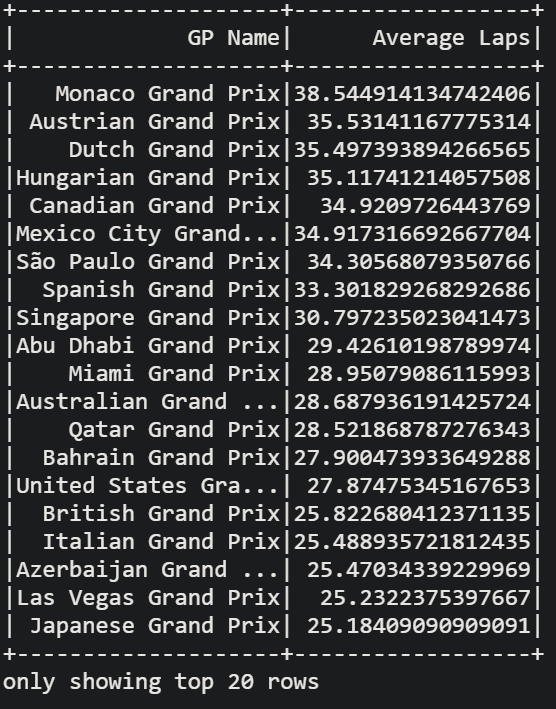
\includegraphics[width=0.6\textwidth]{ss-average-laps.png}
    \caption{Number of Laps GCP Querie Result}
\end{figure}

\begin{figure}[H]
    \centering
    %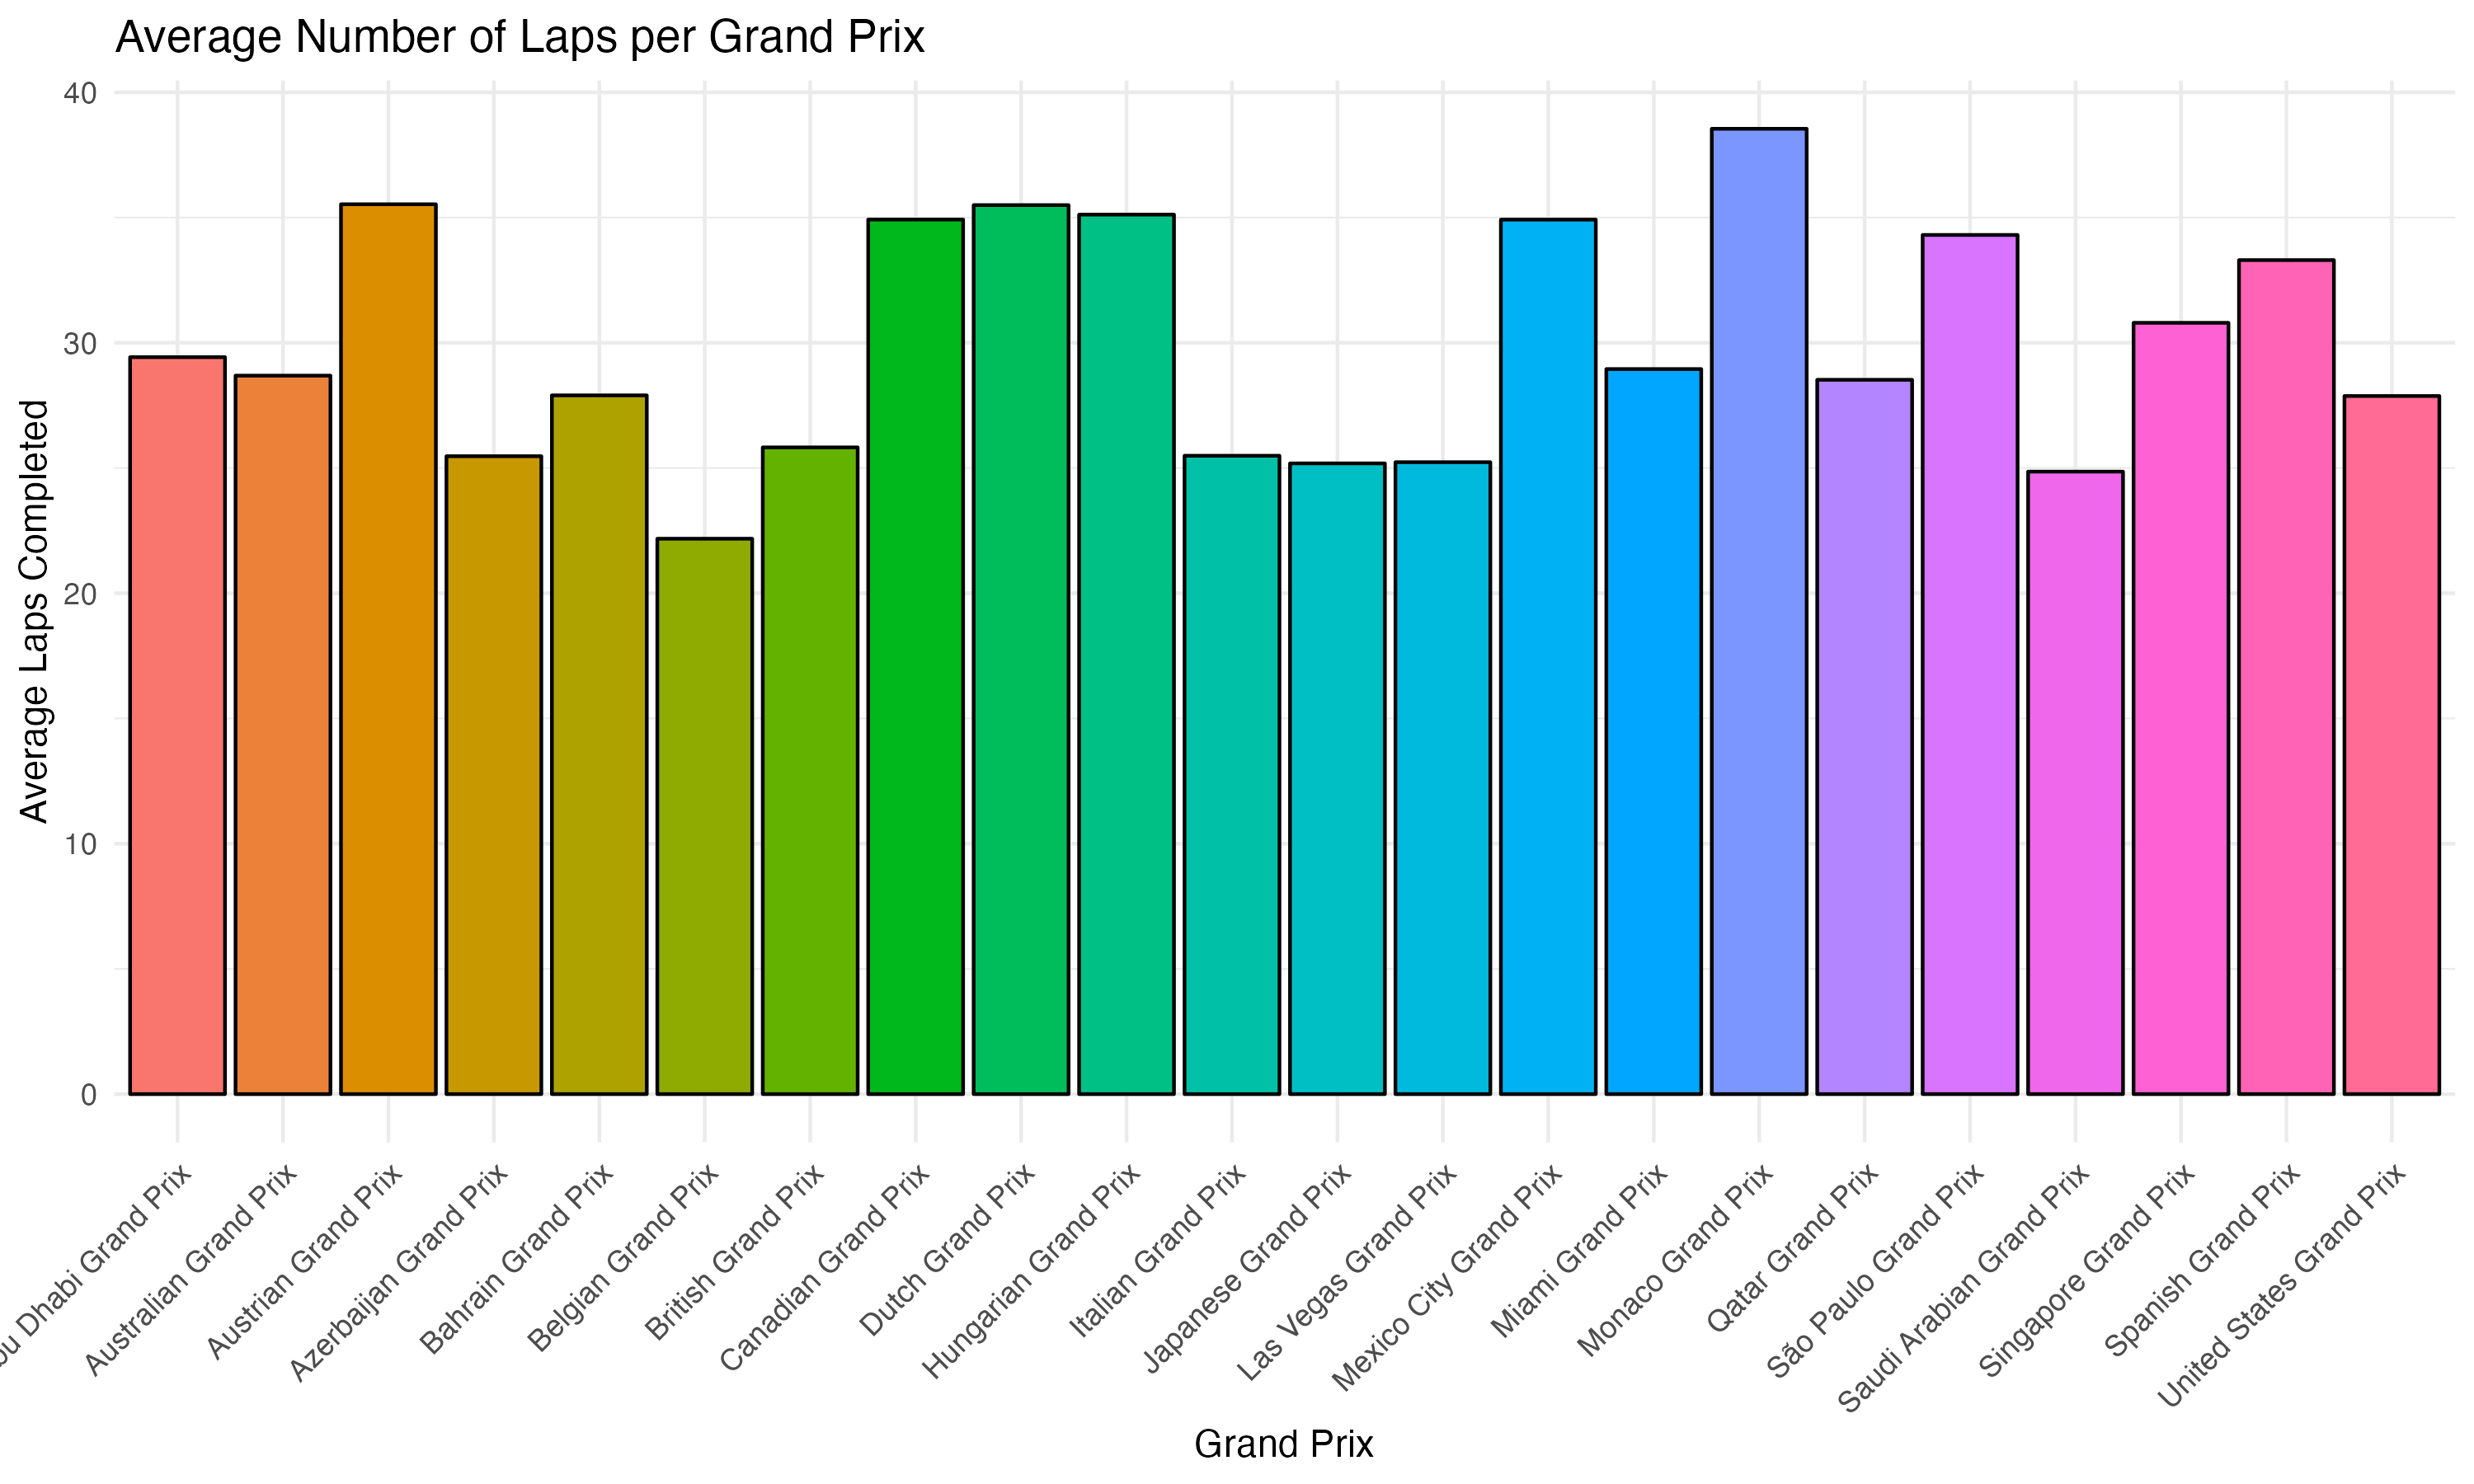
\includegraphics[width=\textwidth]{average_laps_per_gp_plot.png}
    \caption{Bar Chart Average Number of Laps per Grand Prix}
\end{figure}

\paragraph{Interpretation:}
The bar graph visually represents the average number of laps for each Grand Prix, sorted in descending order. Longer races may indicate a need for different tire strategies or fuel management plans. Conversely, shorter races might lead to more aggressive racing tactics. We can say that Monaco GP is the longest and Belgian GP is the shortest with a difference of around 16 laps.


\section{Challenges Encountered}
During the development and analysis phases of our project, we encountered several challenges that fell into two main categories: infrastructure-related and query/code-related. Below, we detail these issues and how we addressed them.

\subsection{Query and Code-Related Challenges}


\section{Conclusions}
Through the utilization of big data technologies such as Hadoop and Hive on the Google Cloud Platform, this project has provided significant insights into the 2023 Formula 1 season. Our comprehensive analysis spanned multiple aspects of the sport, from individual driver performance and tire strategies to the influence of weather conditions on race dynamics.

\paragraph{Insights and Impact:}
The queries conducted revealed:
\begin{itemize}
    
\end{itemize}


\paragraph{Future Directions:}


\paragraph{Final Thoughts:}




\section{Project Repository}
\url{https://github.com/enriquegomeztagle/BigData/tree/main/FinalTerm/F1-GridGuru-Project}

\section{References}
\label{sec:references}


\end{document}
